\section{Design and Implementation}
\label{sec:implementation}
In the following I will present a bunch of noteworthy implementation details. First of all, the implementation is done in \textit{Scala\footnoteUrl{http://www.scala-lang.org/}} (because the DBpedia extraction framework is written in Scala as well), but by the nature of Scala, extensions can also be written in Java or any other JVM language. 
The source code is available via the official DBpedia Mercurial repository\footnoteUrl{http://dbpedia.hg.sourceforge.net/hgweb/dbpedia/extraction_framework/} in the \texttt{wiktionary} branch.

\subsection{Extraction Templates}\label{sec:extpl}
As mentioned in Section~\ref{sec:wiktionary}, we define a \textit{block} as the part of the hierarchical page that is responsible for a certain entity in the extracted RDF graph. 
For each \textit{block}, there can be declarations on how to process the page on that level.
This is done by so called \textit{extraction templates} (called \textit{ET}; not to be confused with the templates of \textit{wikitext}).
Each possible section in the \wik page layout (i.e. each linguistic property) has an ET configured (explained in detail below). 
The idea is to provide a declarative and intuitive way to encode \textit{what to extract}.
For example consider the following page snippet:
\begin{lstlisting}
===Synonyms===
* [[building]]
* [[company]]
\end{lstlisting}
Since the goal is to emit a triple for each link per line, we can write the ET in the following style:
\begin{lstlisting}
===Synonyms===
(* [[\$target]]
)+
\end{lstlisting}
Lets analyse what features are available to build ET.\newline
\textbf{Template matching:}
To match a template against a page, the VarBinder is employed by the Extractor. Page and template are compared node by node:
\begin{figure}[h]
\centering
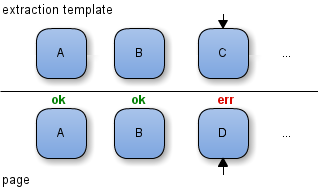
\includegraphics[width=0.4\textwidth]{../images/matching}
\caption{Matching a extraction template against a page}
\label{fig:matching}
\end{figure}
Internally a \texttt{Stack}\footnoteUrl{http://www.scala-lang.org/api/current/scala/collection/mutable/Stack.html} is used; if the head nodes of both stacks are equal, they are consumed, if not an \texttt{Exception} is thrown to notify about a mismatch.\newline
\textbf{Variables:}
In the extraction template, there can be special nodes (e.g. variables). 
If a variable is encountered, all nodes from the page are being recorded and saved as a binding for that variable. 
All bindings that are saved within a extraction template are collected and returned as a result of the template being matched against the page.
\begin{figure}[h]
\centering
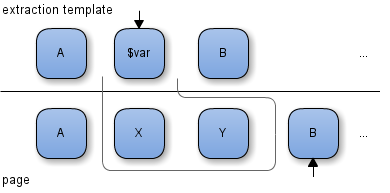
\includegraphics[width=0.4\textwidth]{../images/varbinding}
\caption{recording a variable}
\label{fig:varbinding}
\end{figure}
Some short notes about variables:
\begin{compactitem}
\item the pattern to recognize them is \texttt{\textbackslash\$[a-zA-Z0-9]}
\item they stop recording the page when they encounter the token, that follows the variable in the extraction template
\item if there is no node following them, they consume everything
\item if they record too many nodes (the whole page), they are assumed to be faulty and an exception is thrown
\end{compactitem}
\textbf{Repetition:}
The possibility to have a subtemplate that can be repeated. 
Delimited by \texttt{(} \ldots \texttt{)} and succeeded with one of three modifiers:
\begin{compactitem}
\item \texttt{*} for \textit{0..n} matches,
\item \texttt{+} for \textit{1..n} matches and 
\item \texttt{?} for \textit{0..1} matches.
\end{compactitem}
How do variables relate to repetitions? If a variable is used in a repetition and bound twice, it doubles the number of varbindings. 
Variables outside the repetition are then duplicated. Formalized: the flattened version of the (directed) \textit{binding tree} is the \textit{set of all paths} starting at the root.
\begin{figure}[htbp]
\centering
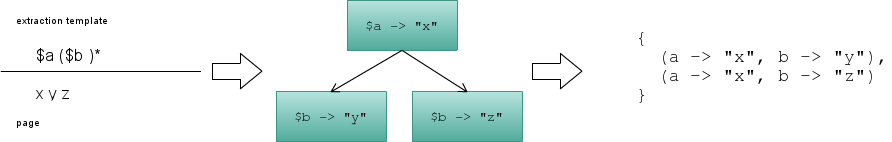
\includegraphics[width=0.8\textwidth]{../images/varlist}
\caption{using variables in repetitions}
\label{fig:varlist}
\end{figure}\newline
\textbf{Error tolerance:}
Due to the human-centric nature of a wiki, pages often contain unexpected information: an additional image, a editor note or a rare template. 
To compensate this, we decided to add the possibility to weaken the conditions for a template mismatch. 
When a node is encountered on the page, that is not expected from the template, the template it is not immediately aborted, but instead it is noted that there was a error and this unexpected node is skipped. 
To limit these skips, a window over the last \textit{s} nodes is observed, to calculate a error threshold \textit{maxError}. 
This allows the template to recover from local errors if it later continues to match. 
Additionally the edge case of templates with length 0 or 1 and 1 unexpected node, should be avoided to succeed by the \textit{minCorrect} parameter that prevents templates from matching too easily.
\begin{figure}[h]
\centering
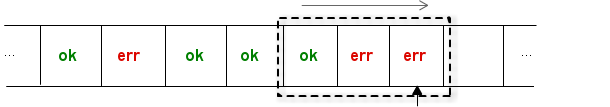
\includegraphics[width=0.8\textwidth]{../images/sliding}
\caption{Error tolerance with a sliding window ($\textit{s}=3, \textit{minCorrect}=1, \textit{maxError}=1)$}
\label{fig:sliding}
\end{figure}
The example shows how confined errors (the single one) are ignored but major errors (like the two consecutive ones) will prevent the template from matching.
This implements a sliding window as only the last \textit{s} nodes are considered and this window progresses with the page being consumed.\newline
These are the most important features of extraction templates.\newline
Back to our example:
The found \textit{variable bindings} are \texttt{\{(\$target -> "building"), (\$target -> "company")\}}. 
How do we transform these bindings into RDF triples? We simply invert the idea of extraction templates to \textit{result templates} (called RT). We insert the value of variables into subject, predicate and object of a RDF triple:
\begin{lstlisting}[style=XML]
<triple s="http://some.ns/$entityId" p="http://some.ns/hasSynonym" o="http://some.ns/$target" />
\end{lstlisting}
Notice the reuse of the \texttt{\$target} variable:
The data extracted from the page is inserted into a triple.
The variable \texttt{\$entityId} is a reserved global variable, that holds the page name i.e. the word.
The created triples in N-Triples syntax are:
\begin{lstlisting}[style=N3]
<http://some.ns/house-1>   <http://some.ns/hasSynonym>   <http://some.ns/building> .
<http://some.ns/house-1>   <http://some.ns/hasSynonym>   <http://some.ns/company> .
\end{lstlisting}
The used RT can be more complex (as explained below).

\subsection{Algorithm}
The algorithm of processing a page works as follows:

\textit{Input:} Parsed page obtained from the DBpedia Framework (essentially a lexer is used to split the Wiki Syntax into tokens)
\begin{enumerate}
\item Filter irrelevant pages (user/admin pages, statistics, list of things, files, templates, etc.) by applying string comparisons on the page title. 
Return an empty set of triples in that case.
\item Build a finite state automaton\footnote{Actually a finite state transducer, most similar to the Mealy-Model.} from the page layout encoded in the WLE specific XML configuration. 
This schema also contains so called \textit{indicator templates} for each \textit{block}, that --- if they match at the current page token --- indicate that their respective block starts. 
So they trigger state transitions. 
In this respect the mechanism is similar to \cite{McCrae_2012}, but in contrast our approach is declarative --- the automaton is constructed \textit{on-the-fly} and not hard-coded. 
The current state represents the current position in the disambiguation tree.
\item The page is processed token by token:
\begin{enumerate}
\item Check if \textit{indicator templates} match. 
If yes, the corresponding block is entered. 
The \textit{indicator templates} also emit triples like in the \textit{extraction template} step below. 
These triples represent the block in RDF -- for example the resource \url{http://wiktionary.dbpedia.org/resource/semantic-English} represents the English block of the page "semantic".
\item Check if any \textit{extraction template} of the current block match.
\subitem If yes, transform the variable bindings to triples.\footnote{In our implementation: 
Either declarative rules are given in the XML config or alternatively static methods are invoked on user-defined classes (implementing a special interface) for an imperative transformation. This can greatly simplify the writing of complex transformation.} Localization specific tokens are replaced as configured in the so called \textit{language mapping} (explained in detail in section \ref{sec:mapping}).
\end{enumerate}
\item The triples are then \textit{transformed}. 
In our implementation \textit{transformation} means, that all triples are handed to a static function, which return a set of triples again. 
One could easily load the triples into a triple store like JENA and apply arbitrary SPARQL Construct and Update transformations. 
This step basically allows post-processing, e.g. consolidation, enrichment or annotation. 
In our case, we apply the schema transformation (by the mediator) explained in detail in Section \ref{sec:lemon}).
\item The triples are sorted and de-duplicated to remove redundancy in the RDF dumps.
\end{enumerate}
\textit{Output:} Set of triples (handed back to the DBpedia Framework).

\subsection{Language Mapping}\label{sec:mapping}
The language mappings are a very simple way to translate and normalize tokens, that appear in a WLE. 
In the German WLE, for example, a noun is described with the German word "\textit{Substantiv}". 
Those tokens are translated to a shared vocabulary, before emitting them (as URIs for example). 
The configuration is also done within the language specific XML configuration:
\begin{lstlisting}[style=XML]
 <mapping from="Substantiv" to="Noun"> 
 <mapping from="Deutsch" to="German"> 
 ...
\end{lstlisting}
The mapping consists currently of mappings for part of speech types and languages. 
But arbitrary usage is possible. 
Section~\ref{sec:functions} shows how this mapping is used.

\subsection{Reference Matching}\label{sec:matching}
A \wik specific requirement is the resolution of intra-page references: All Wiktionaries use \textit{some} way to refer to parts of the traits of the word. 
For example on the page \textit{house} at first senses are defined:
\begin{lstlisting}[basicstyle=\tiny\ttfamily]
# A structure serving as an [[abode]] of human beings.
# {{politics}} A deliberative assembly forming a component of a legislature, or, more rarely, the room or building in which such an assembly normally meets.
# [[house music|House music]].
\end{lstlisting}
Later on relations to other words are noted --- but \textit{in context} of a sense. 
For example house \textit{in context} of \textit{abode} has the translation \textit{Haus} in German. So the following notion is used:
\begin{lstlisting}[basicstyle=\tiny\ttfamily]
====Translations====
{{trans-top|abode}}
...
* German: {{t+|de|Haus|n}}, {{t+|de|Häuser|p}}
...
\end{lstlisting}
The problem is to match the gloss that is given in the \texttt{trans-top} template argument against the available senses.
The senses have been asigned URIs already; now those are needed to serve as subject for the translation triples. There is no simple way to determine which sense URI belongs to which gloss. 
As described in \cite{meyer_2011b} as \textit{relation anchoring}, a string based measure is used\footnote{Opposed to the approach described in \cite{meyer_2011b}, we try to focus on explicit information. Determining the sense URI of a translation triple is already error prone, but so called \textit{target anchoring} is not performed. 
\textit{Target anchoring} refers to the disambiguation of the target word (or entity): this target of course has also a disambiguation tree, and it is possible to \textit{bend} the link to point to a node deeper in that tree instead of just the root node. 
We consider this highly assumptious and it introduces noise. 
We leave that to postprocessing. 
Also it is not implementable easily within the DBpedia framework, because data extracted on other pages is not available to a extractor at runtime.}. 
There is a simple data structure that is initialized per page, to this matching mechanism. Which measure is used can be configured in the global configuration. 
Available measures are: Levenshtein and trigram set similarity with dice, jaccard or overlap coefficient. 
A sense can be registered with the matcher by passing its definition sentence. 
An \textit{id} is generated for that sense. 
Later on, glosses (short forms of the definition) that refer to a sense can be passed to lookup which sense matches best, and the corresponding \textit{id} is returned. 
Opposed to existing approaches we make no assumptions on how such references are noted. 
The English \wik uses glosses, the German one uses explicit numbers (that don't need to be matched), the Russian and French uses a combination of both --- sometimes senses are explicitly referred to by their numbers, sometimes with a gloss. 
So we came up with a customizable way to use the reference matcher. 
Section~\ref{sec:functions} shows how this mechanism is used.

\subsection{Formatting functions in Result Templates}\label{sec:functions}
The question arises, how this mapping is then used within the application. 
It is certainly not reasonable to replace \textit{all} occurrences of those \texttt{from} tokens. This would lead to a number of false positive matches and screwed output. 
It is crucial to offer a possibility to configure in which context output should be handled so.
I therefore introduced formatting functions in result templates: when you note the triples that are generated you can apply functions to e.g. variables. 
An example:
\begin{lstlisting}[style=XML]
<triple s="http://some.ns/uri($entityId)" p="http://some.ns/hasLanguage" o="http://some.ns/map($target)" />
\end{lstlisting}
In this RT, two functions are used: \texttt{uri} and \texttt{map}. 
They are wrapped around variable parts, and on rendering they are resolved. 
The following functions are available:\\
\begin{table}[h!] 
\centering 
\begin{tabular}{|l|l|}
\hline \texttt{uri(str)} & URL encode \\ 
\hline \texttt{map(str)} & replace if mapping found \\ 
\hline \texttt{assertMapped(str)} & dont emit triple if not in mapping vocabulary \\ 
\hline \texttt{assertNumeric(str)} & dont emit triple if argument is not numeric \\ 
\hline \texttt{getId(str)} & lookup a gloss and return the id of the best matching sense \\ 
\hline \texttt{getOrMakeId(str)} & lookup a id or generate one if below a similarity threshold \\ 
\hline \texttt{makeId(str)} & save a sense and generate an id \\ 
\hline \texttt{saveId(str, str)} & save a sense with a given id \\ 
\hline 
\end{tabular} 
\end{table}
The functions with \textit{Id} in their name relate to the matching introduced in section~\ref{sec:matching}. 
Continuing the example of senses and translations, one would write the RT in a way to save definition sentences when generating them as triples and later matching the gloss, when generating triples about the translation section:
For the defintions
\begin{lstlisting}[style=XML]
<triple s="http://some.ns/$entityId-makeId($definition)" p="http://some.ns/hasDefinition" o="$definition" oType="literal" />
\end{lstlisting}
and for the translations
\begin{lstlisting}[style=XML]
<triple s="http://some.ns/$entityId-getId($gloss)" p="http://some.ns/hasTranslation" o="http://some.ns/uri($target)" />
\end{lstlisting}
The idea is that (if the matching is correct), the subject URIs are equal (e.g. \url{http://some.ns/house-1}) in both triples --- there are two triples about one resource --- information successfully merged.
\begin{lstlisting}[style=N3]
<http://some.ns/house-1>   <http://some.ns/hasDefinition>   "A structure serving as an abode of human beings." .
<http://some.ns/house-1>   <http://some.ns/hasTranslation>   <http://some.ns/Haus> .
\end{lstlisting}
 
\subsection{Schema Mediation by Annotation with \lemonnospace}
\label{sec:lemon}
The last step of the data integration process is the schema normalization.
The global schema of all WLE is not constructed in a centralized fashion --- instead we found a way to both making the data globally navigable and keeping the heterogeneous schema without loosing information.
\lemonnospace~\cite{lemon-eswc} is an RDF model for representing lexical information (with links to ontologies --- possibly DBpedia). 
We use part of that model to encode the relation between \textit{lexical entries} and \textit{lexical senses}.
\lemon has great potential of becoming the \textit{de facto} standard for representing dictionaries and lexica in RDF and is currently the topic of the OntoLex W3C Community group\footnote{\url{http://www.w3.org/community/ontolex/}}. 
The rationale is to add \textit{shortcuts} from \textit{lexical entities} to \textit{senses} and propagate properties that are along the intermediate nodes down to the senses.
This can be accomplished with a generic algorithm (a generic tree transformation, regardless of the depth of the tree and used links).
Applications assuming only a \textit{lemon} model, can operate on the shortcuts and (if applied as an overlay --- leaving the original tree intact) this still allows applications, to also operate on the actual tree layout.
The (simplified) procedure is presented in Figure~\ref{fig:lemon}\footnote{Note, that in the illustration it could seem like the information about part-of-speech would be missing in the \textit{lemon} model. This in not the case. Actually from the part-of-speech nodes, there is a link to corresponding language nodes.
These links are also propagated down the tree.}. 
\begin{figure}[tb]
\centering
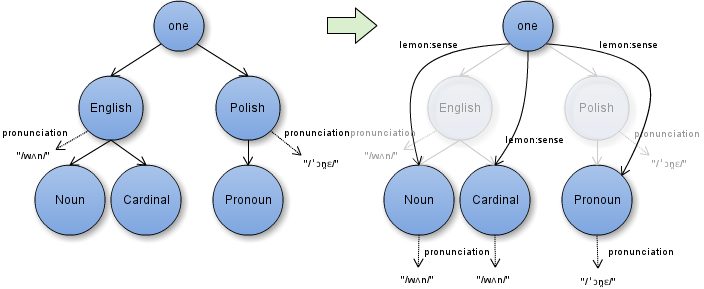
\includegraphics[width=\textwidth]{./images/lemon.png}
\caption{Schema normalization.}
\label{fig:lemon}
\end{figure}
The use of the \lemon vocabulary and model as an additional schema layer can be seen as our mediator.
This approach is both lightweight and effective as it takes advantage of \textit{multi-schema modelling}.

\subsection{Configuration}
As presented in section \ref{sec:requirements}, the most important requirement of the approach is configurability. The extractor itself is as generic as possible, it is not tailored to linguistics or even \wik. 
It has commitment to wiki syntax, but is also able to process plain text as it can be interpreted as wikitext without markup, thus the extractor may be suitable for most flat file formats. 
However the configuration makes up the heart of the extractor: it is a big XML file interpreted at runtime and describes how to interpret the page. 
I will go through the available options and show their relevance to the given requirements.

At first the configuration is splitted into a generic part and a language specific part. 
The generic part is always loaded and does not need to be localized to a WLE. 
It contains options like the namespace, in which all URIs are created and an option that specifies which language configuration should be used. 
The language specific configuration is loaded based on that option at runtime. 
It has to be tailored to a WLE by the maintainer of the dataset.

Both configuration types are stored in the \texttt{config} folder. 
The naming convention restricts the folder to like the following:
\dirtree{%
.1 config.
.2 config.xml.
.2 config-de.xml.
.2 config-en.xml.
.2 \ldots.
}

The generic configuration has two parts: a properties list and a mapping. 
The properties are the mentioned namespace, the language, the \texttt{loglevel} (to configure debug verbosity) and options to configure the matcher. 
The mapping is --- as explained in section~\ref{sec:mapping} --- a way to replace tokens found on the page to a global vocabulary. 
But opposed to language specific tokens, in the generic configuration, globally used tokens are configured. 
It is used to provide a mapping from ISO 639-1 and -2 codes to the \wik vocabulary.

\begin{lstlisting}[style=XML]
<?xml version="1.0" encoding="UTF-8"?>
<config>
    <properties>
        <property name="logLevel" value="0"/>
        <property name="language" value="ru"/>
        <property name="ns" value="http://wiktionary.dbpedia.org/"/>
        <property name="matchingStrategy" value="levenshtein"/>
        <property name="matchingThreshold" value="0.5"/>
    </properties>
    <mappings>
        <!-- ISO 639-1 -->
        <mapping from="aa" to="Afar" />
        <mapping from="ab" to="Abkhazian" />
        <mapping from="ae" to="Avestan" />
        ...
\end{lstlisting}

The language specific configuration is probably the most important part of this thesis. 
The created XML dialect directly reflects the expressiveness of the extraction approach. 
As explained in section \ref{sec:requirements}, the expressiveness is limited by the complexity of the declarative language. 
However he declarative language should remain simple to keep it easily usable by non experts. 
The interpreter should be as generic as possible. 
In the following I will present which trade off was chosen and how the layout of a WLE is modelled in our XML dialect.

The configuration for English should serve as an example here\footnoteUrl{http://dbpedia.hg.sourceforge.net/hgweb/dbpedia/extraction_framework/file/c871ba718cf6/wiktionary/config/config-en.xml}. 
The XML is structured as
\dirtree{%
.1 <config>.
.2 <ignore>.
.2 <mappings>.
.2 <postprocessing>.
.2 <saveVars>.
.2 <templateRepresentativeProperties>.
.2 <page>.
}

The \texttt{<ignore>} section configures which pages shall be skipped and not used for extraction. 
This is used to skip help pages or user profiles, but it can be also used to skip pages like conjugation tables, as they are not handled yet. 
An example for this section could be
\begin{lstlisting}[style=XML]
<ignore>
	<page startsWith="Help:" />
	<page endsWith=" (Conjugation)" />
	...
\end{lstlisting}
There are two options to determine if a page should be skipped: Prefix or suffix matches in the page title.

The mappings section has been explained in \ref{sec:mapping}, it is used to translate language specific terms for languages or part of speech types and can be invoked by formatting functions in result templates as explained in \ref{sec:functions}.\newline
\texttt{<postprocessing>} configures whether and how the extracted triples of a page should be handled. 
It is possible to pass them to so called \texttt{Postprocessors} (that are JVM classes, visible in classpath, that need to implement a certain interface \texttt{Postprocessor}). 
This \texttt{Postprocessor} can be configued by arbitrary XML nodes. 
The interpretion of those is left to the class itself. 
An example for \texttt{Postprocessors} is the lemon overlay. 
It is invoked like this:
\begin{lstlisting}[style=XML]
<postprocessing enabled="true" ppClass="org.dbpedia.extraction.mappings.wikitemplate.wiktionary.postprocessor.LemonOverlay">
  <config>
    <blockProperty uri="http://www.monnet-project.eu/lemon#sense"/>
    <inputTargetClass uri="http://wiktionary.dbpedia.org/terms/Sense"/>
    <followProperties>
      <property uri="http://wiktionary.dbpedia.org/terms/hasPoSUsage"/>
      <property uri="http://wiktionary.dbpedia.org/terms/hasLangUsage"/>
      <property uri="http://wiktionary.dbpedia.org/terms/hasSense"/>
    </followProperties>
    <collectProperties>
      <property uri="http://purl.org/dc/elements/1.1/language"/>
      <property uri="http://www.w3.org/2000/01/rdf-schema#label"/>
      <property uri="http://wiktionary.dbpedia.org/terms/hasMeaning"/>
      <property uri="http://wiktionary.dbpedia.org/terms/hasTranslation"/>
      <property uri="http://wiktionary.dbpedia.org/terms/hasExampleSentence"/>
      ...
    </collectProperties>
    <outputStartClass uri="http://www.monnet-project.eu/lemon#LexicalEntry"/>
    <outputAggregatedClass uri="http://www.monnet-project.eu/lemon#LexicalSense"/>
  </config>
</postprocessing>
\end{lstlisting}

\texttt{<saveVars>} allows to cache variables between template matches. 
Normally the only variables visible in result templates, are the ones bound in the extraction templates. 
We extended this with a cache, so certain variables can be kept. 
If a variable is set to be saved like this
\begin{lstlisting}[style=XML]
<saveVars>
  <var name="pos"/>
  <var name="language"/>
  <var name="definition"/>
</saveVars>
\end{lstlisting}
its last value stays available to be used in further result templates. In other words: after being bound, the variable stays visible --- gets a global scope. 
This memory allows for a kind of context sensitivity by means of \textit{look back}. 
The mechanism is currently not used.\newline
\texttt{templateRepresentativeProperties} works as a very simple \textit{template resolution} mechanism. 
To resolve templates (render them to readable text), actually a running MediaWiki instance is necessary. 
But often this is superfluous: it might be sufficient to simply choose a argument of that template to represent it readable. 
For example the English template \texttt{term} is used to format links to other words; it is printed as the word itself which is the first argument. 
Other information can be ignored. 
So I came up with this simple but effective mechanism to note which property is used to represent templates:
\begin{lstlisting}[style=XML]
<templateRepresentativeProperties>
  <templateRepresentativeProperty tplName="term" pKey="1"/>
  ...
  <templateRepresentativeProperty tplName="proto" pKey="2"/>
</templateRepresentativeProperties>
\end{lstlisting}

Finally we come to the most important section: the \texttt{page} section. 
It describes the overall layout of a page within a WLE.
As defined in section~\ref{sec:wiktionary}, a page is hierarchically divided into \textit{blocks}. 
The need arises to configure
\begin{enumerate}
\item the hierarchy of the blocks
\item how the start of a block is recognized
\item which extraction templates are used in each block
\end{enumerate}

The first is achieved by nesting \texttt{<block>} nodes into each other:
\begin{lstlisting}[style=XML]
<page>
  <block name="language">
    <block name="pos>
      ...
    </block>
  </block>
</page>
\end{lstlisting}

The second is realised by reusing templates. 
As introduced above, templates are matched against the page; additionally to extracting triples, they are here used to react \textit{when} they match. 
A block can have several templates configured and while the extractor scans the page, it tries to match these \textit{indicator templates}.
If they match, they trigger the start of a block. In the next step we will see how such a template is actually configured. 
The syntax for extraction templates and indicator templates is exactly the same\footnote{the interpreting code is reused}. 
The indicator templates are stored in each block:
\begin{lstlisting}[style=XML]
<block name="language">
  <indicators>
    <indicator>
      ... (see below)
    </indicator>
  </indicators>
  ...
</page>
\end{lstlisting}

The third is done by the \texttt{templates} section within each block:
\begin{lstlisting}[style=XML]
<block name="language">
  <indicators />
  <templates>
    <template name="example">
      <wikiTemplate>===Etymology=== 
$etymology
</wikiTemplate>
      <resultTemplates>
        <resultTemplate>
          <triples>
            <triple s="$block" p="http://wiktionary.dbpedia.org/terms/hasEtymology" o="$etymology" oType="literal"/>
          </triples>
        </resultTemplate>
      </resultTemplates>
      </template>
    </template>
  </templates>
</page>
\end{lstlisting}
The basics were explained in section~\ref{sec:extpl}, now we put them together: the \texttt{<template>} node is divided into two parts --- the extraction template in \texttt{<wikiTemplate>} and the result templates.

The \textit{extraction template} has been explained already above. 
It is put in the \texttt{<wikiTemplate>} node --- only thing to keep in mind there is whitespace: whitespaces count, also every indention or linebreak will be interpreted as wiki text. 
Make sure you don't accidentally change the template, because it will most likely not match anymore.
Also set your text editor to show control characters like spaces, tabs, or newlines (cf. the $\P$ symbol).

Additionally to the \textit{result template} basics introduced above, for a \texttt{<template>} there can be multiple RT and each consist of a set of triple templates. 
The rational is to respect missing bindings: if a variable is inside a optional repetition, it may not be present in the variable bindings. 
If those bindings are then converted to triples by a \textit{result template}, missing variables will result in the current triple to fail. 
To avoid inconsistent triples (because some are missing), then all triples shall not be emitted. 
Thus result templates are atomic --- either all triples inside are emitted or none. 
This allows to model triples separately for varying page content \textit{within one template}.
Another way to respect diverse layouts, is to declare a triple \textit{optional}:
\begin{lstlisting}[style=XML]
<resultTemplate>
  <triple s="http://some.ns/$entityId" p="http://some.ns/hasSense" o="http://some.ns/$entityId-$sense" />
  <triple s="http://some.ns/$entityId-$sense" p="http://some.ns/hasSource" o="$source" optional="true" />
</resultTemplate>
\end{lstlisting}
This disregards a missing variable --- the result template will still succeed if the optional triple fails.

A very important feature is the global \texttt{\$block} variable together with the \texttt{oNewBlock} configuration option within \textit{indicator templates}:
Global variables have already been introduced by the \texttt{\$entityId} variable and the possibility to save variables between templates. 
The \texttt{\$entityId} variable is static, it keeps it value over time. 
Saved variables are local variables that become global. 
Now we introduce the \texttt{\$block} variable, that holds the URI of the current block. 
For example if the extractor currently processes the language block of a word the value could be \url{http://some.ns/Haus-German}. 
This value can then be used to construct URIs that reuse this as a prefix:
\begin{lstlisting}[style=XML]
<triple s="$block" p="http://some.ns/hasPosUsage" o="$block-$pos" oNewBlock="true" />
\end{lstlisting}
The object URI could be \url{http://some.ns/Haus-German-Noun} for example. 
But furthermore, if this RT is used within an \textit{indicator template}, the need arises to indicate the start of a new block. 
When I introduced \textit{indicator templates} above --- i lied: not the successful match of template triggers the state change, but only the successful rendering of its result template, including a triple with the \texttt{oNewBlock} option.
The rational is, that to trigger that transition, the new block URI has to be known --- and there is no simple way to determine it from a set of unremarkable triples that are produced by the indicator template.
Of course the \texttt{\$block} variable can be used independently from the \texttt{oNewBlock} option in ordinary RT.

\subsection{Utility Tools}
To provide a complete deployment environment for the Wiktionary RDF dataset, it is also necessary to cater for tools to \textit{load} the data into a database. We chose \textit{Virtuoso} for this purpose and I created a set of tools that relate to data loading (and cleaning).

\begin{footnotesize}
\begin{tabular}{|p{0.1\textwidth}|p{0.1\textwidth}|p{0.1\textwidth}|p{0.6\textwidth}|}
\hline \textbf{script} & \textbf{parameters} & \textbf{result} & \textbf{note} \\ 
\hline splitrapper & <nt-file> & cleaned nt-file & splits a nt-file into parts, small enough for \textit{rapper} (part of the libraptor utils), to process it (the current implementation of rapper has a limit at 2GB). Applies rapper to each part to clean common encoding problems and concatenates the cleaned parts back together \\ 
\hline virtuoso-load & <init> <lc>+ & loaded language dumps in Virtuoso & init (either "true" or "false") specifies whether the database should be purged first. Then for each language code, the corresponding nt-file is loaded into Virtuoso, while setting up the graph layout accordingly. \\
\hline publish-download & <lc>+ & nt-files uploaded &  expects passwordless \texttt{ssh} access to the DBpedia download server, \texttt{gzip}s them, uses \texttt{scp} to upload the files and names them with the current date.\\
\hline make\_jarzip & - & executable jar file of the extractor & creates a zip file that contains a executable jar of the wiktionary source code, containing all dependencies (to the framework and to configuration resources). Enables the easy distribution of the software for people without Mercurial knowledge.\\
\hline statistics & <nt-file> & printed statistics & generates statistics about a nt-file (e.g. triple count, property usage, sense counts)\\
\hline translation-extract & - & translations CSV file & retrieves all translation pairs from a SPARQL endpoint and serializes them in a fixed CSV format. The translation source word is disambiguated by language, part of speech and sense.\\
\hline translation-loader.sql & - &  & execute from SQL console to load CSV file into a fixed SQL table \\
\hline 
\end{tabular} 
\end{footnotesize}

The first four are used for deployment, the statistics tool is informative and the last two are descended from a specific use case that can also serve as a best practice for similar tasks. The task in this case was to export translations to a relational schema. I choose to do it via CSV as an intermediate step, as this format is both easy to serialize and easy to load from SQL. If the need arises to do something similar (for example with synonyms), this script is easy to adapt.

\subsection{Graph Layout}

\newpage

